\documentclass[a4paper,12pt]{article}
\usepackage[utf8]{inputenc}
\usepackage[T1]{fontenc}
\usepackage{lmodern}
\usepackage{geometry}
\usepackage{setspace}
\usepackage{fancyhdr}
\usepackage{hyperref}
\usepackage{amsmath}
\usepackage{amsfonts}
\usepackage{amssymb}
\usepackage{mathtools}
\usepackage{float}
\usepackage{tabularx}
\usepackage{enumitem}
\usepackage{graphicx}
\usepackage{ragged2e}
\usepackage[spanish]{babel}
\usepackage{booktabs}
\usepackage{longtable}
\usepackage{multirow}
\usepackage{xcolor}
\usepackage{microtype}
\usepackage{caption}
\usepackage{textcomp}
\newcommand{\euro}{\texteuro}
\newcommand{\E}{\mathbb{E}}
\newcommand{\Var}{\mathrm{Var}}
\newcommand{\Cov}{\mathrm{Cov}}
\newcommand{\VaR}{\mathrm{VaR}}
\newcommand{\TVaR}{\mathrm{TVaR}}
\addto\captionsspanish{\renewcommand{\tablename}{Tabla}}
\addto\captionsspanish{\renewcommand{\figurename}{Figura}}
\captionsetup{font=small,labelfont=bf}

% Configuración de márgenes
\geometry{left=2.5cm,right=2.5cm,top=3cm,bottom=3cm}

% Configuración de encabezados y pies de página
\pagestyle{fancy}
\fancyhf{}
\renewcommand{\headrulewidth}{0pt}
\fancyfoot[C]{\thepage}

% Configuración de interlineado
\onehalfspacing
\justifying

% Configuración de hipervínculos
\hypersetup{
    hidelinks,
    colorlinks=false
}

\begin{document}

% Primera página (Título, Resumen y Abstract)
\begin{titlepage}
    \centering
    \vspace*{0.1cm}
    \huge\textbf{Tema 3: Preguntas de debate}\\
    \vspace{1cm}
    \small{Luiz Alberto Luzuriaga Izquierdo}\\
    \vspace{0.1cm}
    Facultad de ciencias económicas, empresariales y turismo. \\
    \vspace{0.1cm}
    Universidad de Alcalá de Henares. \\
    \vspace{0.1cm}
    Curso 2026-2027\\
    \vspace{0.5cm}

{\bfseries Resumen}

\vspace{0.1cm}
\noindent
\begin{justify}
Respuestas argumentadas a las preguntas de debate del tema, con cifras de los casos prácticos. Tema 3 (Modelo colectivo de riesgo): Frecuencia y severidad, recursión de Panjer y FFT, sobredispersión y colas pesadas.\\\\
\vspace{0.1cm}
\noindent
\textbf{Palabras clave}: modelo colectivo, frecuencia, severidad, Panjer, preguntas de debate.
\end{justify}
\begin{center}
    {\bfseries Abstract}
\end{center}
\vspace{0.1cm}
\noindent
\begin{justify}
Class work for Topic 3 of Actuarial Mathematics of Stability and Solvency of Insurance Activity: discussion questions with actuarial reasoning and numerical evidence.\\\\
\vspace{0.1cm}
\noindent
\textbf{Keywords}: collective risk model, frequency, severity, Panjer, discussion questions.
\end{justify}

\end{titlepage}

% Índice
\newpage\pagenumbering{gobble}
\renewcommand{\contentsname}{Índice}
\newgeometry{left=4cm, right=4cm, top=3cm, bottom=2.5cm}
\tableofcontents

\restoregeometry
\newpage
\numberwithin{equation}{section}
\pagenumbering{arabic}
\setcounter{page}{1}

\section{Tema 3: Modelo colectivo de riesgo}
\label{sec:tema3debate}
\noindent
Respuestas argumentadas a las preguntas de debate del tema, con cifras de los casos prácticos. Material de referencia: diapositivas del Tema 3 (Prof. Hugo González Riera).

\subsection{Debate 1 -- ?`C\'omo detectar sobredispersi\'on y decidir entre Poisson y Binomial Negativa?}

\paragraph{Tesis.} No basta con mirar un n\'umero: se combinan un diagn\'ostico descriptivo, un contraste formal y una comparaci\'on de modelos, y despu\'es se investiga \emph{por qu\'e} hay sobredispersi\'on.

\paragraph{Datos.} Se necesitan recuentos de siniestros por unidad de observaci\'on (p\'oliza-a\~no) y su exposici\'on. Antes de nada hay que normalizar por la exposici\'on: si unas p\'olizas est\'an un mes y otras doce, una Poisson con \emph{offset} $\log(\text{exposici\'on})$ evita confundir exposici\'on diferente con sobredispersi\'on.

\paragraph{Procedimiento.}
\begin{enumerate}[leftmargin=*,itemsep=2pt]
\item \textbf{\'Indice de dispersi\'on.} $\hat\phi=s^2/\bar y$ con $s^2$ la varianza muestral. Bajo Poisson $\phi=1$. Es el primer filtro y una pista de la magnitud: $\phi=1+\beta$ en la BN.
\item \textbf{Contraste de la $\chi^2$ de dispersi\'on.} Bajo $H_0$ (Poisson), $(n-1)\,s^2/\bar y\sim\chi^2_{n-1}$ aproximadamente. En el an\'alisis sobre un entorno de regresi\'on, el estad\'istico de Pearson $\sum(y_i-\hat\mu_i)^2/\hat\mu_i$ dividido por los grados de libertad debe estar cerca de 1, o el test auxiliar de Cameron y Trivedi (regresi\'on de $\big((y_i-\hat\mu_i)^2-y_i\big)/\hat\mu_i$ sobre $\hat\mu_i$).
\item \textbf{Raz\'on de verosimilitudes Poisson vs BN.} $LR=2(\ell_{NB}-\ell_{Pois})$. Como $r\to\infty$ (Poisson) est\'a en la frontera del espacio de par\'ametros, el $p$-valor es el de una mezcla $\tfrac12\chi^2_0+\tfrac12\chi^2_1$, es decir, $\tfrac12P(\chi^2_1>LR)$.
\item \textbf{Criterios de informaci\'on y ajuste.} Comparar AIC/BIC y, sobre todo, los recuentos observados frente a los esperados por cada modelo (cola de frecuencias altas).
\end{enumerate}

\paragraph{Ejemplo (simulaci\'on del tema).} 20.000 p\'olizas con tasa individual aleatoria $\Lambda\sim\text{Gamma}$ de media $0{,}15$ (heterogeneidad no observada):
\begin{center}
\begin{tabular}{lr}
\toprule
Media $\bar y$ & $0{,}1514$\\
Varianza $s^2$ & $0{,}2024$\\
\'Indice de dispersi\'on $s^2/\bar y$ & $1{,}337$\\
$\chi^2$ (19.999 g.l.) & $26.738$, $p\approx10^{-205}$\\
BN por MLE & $\hat r=0{,}453$, $\hat\mu=0{,}1514$\\
$LR=2(\ell_{NB}-\ell_{Pois})$ & $587{,}1$ ($\ell$: $-8.910{,}1$ frente a $-9.203{,}6$), $p\approx10^{-130}$\\
AIC & Poisson $18.409{,}3$; BN $17.824{,}2$\\
\bottomrule
\end{tabular}
\end{center}
\begin{center}
\begin{tabular}{rrrr}
\toprule
$n$ siniestros & Observado & Poisson & Bin. Negativa\\
\midrule
0 & 17.551 & 17.191 & 17.552\\
1 & 1.997 & 2.602 & 1.991\\
2 & 352 & 197 & 362\\
3 & 82 & 10 & 74\\
4 & 11 & 0 & 16\\
5 & 6 & 0 & 4\\
\bottomrule
\end{tabular}
\end{center}
La Poisson infravalora las colas de frecuencia (82 p\'olizas con 3 siniestros frente a 10 esperadas); la BN las reproduce.

\paragraph{Por qu\'e puede aparecer sobredispersi\'on (y c\'omo reaccionar).}
\begin{itemize}[leftmargin=*,itemsep=1pt]
\item \textbf{Heterogeneidad no explicada} entre asegurados $\Rightarrow$ a\~nadir variables tarifarias; si la sobredispersi\'on persiste tras el GLM, usar BN (mezcla Poisson--Gamma).
\item \textbf{Exposici\'on mal medida o siniestros agrupados} (un mismo evento genera varios partes) $\Rightarrow$ definir bien la unidad (evento frente a siniestro).
\item \textbf{Factores comunes de a\~no} (clima, inflaci\'on) $\Rightarrow$ no se resuelve con m\'as variables individuales; es riesgo sistem\'atico que debe entrar en el capital.
\item \textbf{Exceso de ceros}: si hay muchos m\'as ceros de los que predice la BN, modelos inflados en cero.
\end{itemize}

\paragraph{Qu\'e cambia en el capital.} Si se usa Poisson con la misma media en Hogar, $\Var(S)$ cae de $9\cdot10^8$ a $4{,}5\cdot10^8$ y el VaR Normal baja de $227.275$ a $204.642$ \euro: un $10\%$ de capital que desaparece solo por haber elegido mal la frecuencia.

\bigskip\hrule\bigskip

\subsection{Debate 2 -- Estructura de exceso de p\'erdida para Hogar}

\paragraph{Tesis.} Un exceso de p\'erdida (XL) \emph{por riesgo} con prioridad entre $5.000$ y $10.000$ \euro\ (de 5 a 10 veces la severidad media) es la pieza principal; hay que completarlo con una cobertura de acumulaci\'on (cat XL o stop-loss) si hay riesgo de evento. Reduce la cola y el capital mucho m\'as de lo que reduce la asimetr\'ia.

\paragraph{Qu\'e hace el XL por riesgo.} Cada siniestro queda limitado a $\min(X,d)$; la parte $(X-d)_+$ la asume el reasegurador, con recobros esperados $\E[N]\,\E[(X-d)_+]=\E[N]\,\frac{\theta}{\alpha-1}\big(\frac{\theta}{\theta+d}\big)^{\alpha-1}$ para la Pareto. Acota la severidad retenida (le da todos los momentos finitos) y por tanto trunca la cola de $S$.

\paragraph{Resultados en la cartera de Hogar} (distribuci\'on exacta por FFT; carga del reasegurador del $30\%$ sobre los recobros esperados; coste de capital del $6\%$ como en el margen de riesgo de Solvencia~II).
\begin{center}
\small
\begin{tabular}{rrrrrrrr}
\toprule
Prioridad $d$ & $\E[S]$ neto & $SD$ & $\gamma_S$ & VaR 99,5\,\% neto & Ahorro de VaR & Prima ($1{,}3\times$ recobros) & Carga m\'axima rentable\\
\midrule
sin XL & 149.917 & 29.993 & 0,397 & 238.300 & -- & -- & --\\
20.000 & 149.584 & 29.608 & 0,354 & 235.600 & 2.700 & 433 & $48{,}6\%$\\
10.000 & 148.073 & 28.772 & 0,332 & 231.000 & 7.300 & 2.396 & $23{,}8\%$\\
5.000 & 142.007 & 26.666 & 0,311 & 218.400 & 19.900 & 10.283 & $15{,}1\%$\\
3.000 & 131.169 & 23.859 & 0,301 & 199.300 & 39.000 & 24.375 & $12{,}5\%$\\
1.500 & 105.483 & 18.421 & 0,293 & 158.000 & 80.300 & 57.778 & $10{,}8\%$\\
\bottomrule
\end{tabular}
\end{center}
La \emph{carga m\'axima rentable} es la carga del reasegurador para la cual el coste de capital liberado ($6\%\times$ ahorro de VaR) iguala al sobrecoste de la carga ($\text{carga}\times$ recobros esperados).
\begin{figure}[H]\centering
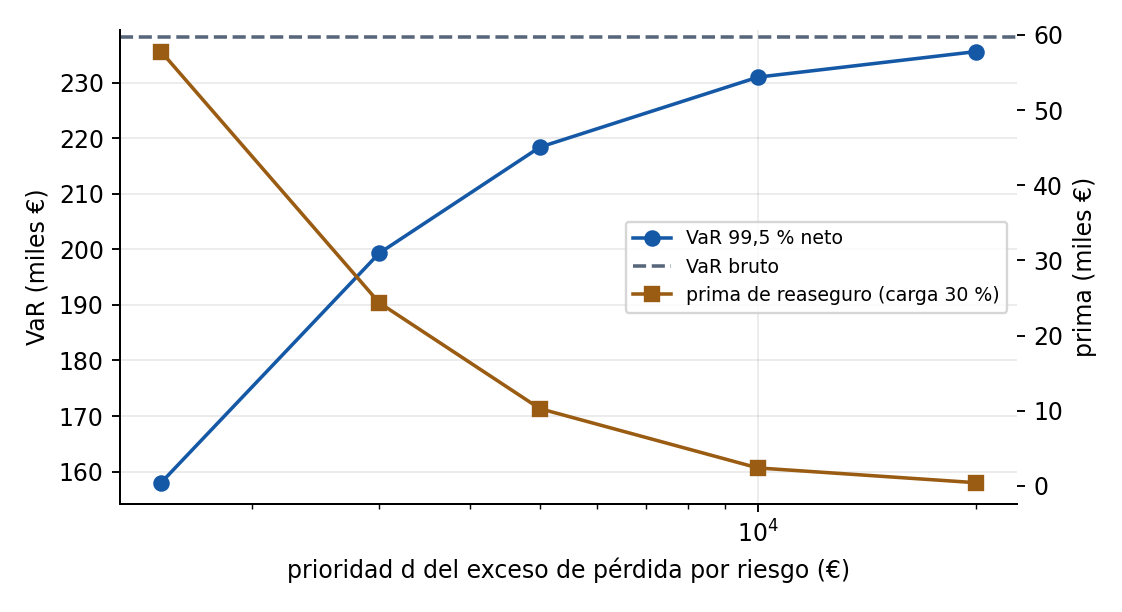
\includegraphics[width=.72\linewidth]{t3_f_debate2.png}
\caption{VaR neto y prima de reaseguro frente a la prioridad $d$ en la cartera de Hogar.}
\end{figure}

\paragraph{Lectura.}
\begin{enumerate}[leftmargin=*,itemsep=2pt]
\item \textbf{El XL reduce el capital mucho m\'as que la asimetr\'ia.} Con $d=5.000$ el VaR baja un $8\%$ ($238.300\to218.400$), pero $\gamma_S$ solo baja de $0{,}40$ a $0{,}31$: en esta cartera la asimetr\'ia viene sobre todo de la frecuencia (con $\E[N]=150$ y factor com\'un de BN) y de la severidad de Pareto moderada, no de unos pocos siniestros enormes. Para la fiabilidad de la aproximaci\'on basta con que ya existan los tres primeros momentos y que se use la Normal Power o el c\'alculo exacto.
\item \textbf{Prioridades altas son baratas por euro de protecci\'on.} Con $30\%$ de carga solo compensa reasegurar por encima de $d\approx5.000$--$10.000$: a $1.500$ la carga m\'axima rentable es $10{,}8\%$ (por debajo de lo que se suele cobrar), a $10.000$ es $23{,}8\%$ y a $20.000$ el ahorro es ya marginal.
\item \textbf{La pieza que falta es el riesgo de acumulaci\'on.} Un XL \emph{por riesgo} no protege contra una tormenta que genera miles de siniestros peque\~nos a la vez (cada uno por debajo de $d$); para ello se contrata un \emph{cat XL por evento} (con prioridad definida sobre la p\'erdida de evento agregada) o un stop-loss agregado.
\item \textbf{Efecto en la cola y en la cuota.} Un XL deja la media de los siniestros peque\~nos al asegurador y transfiere el riesgo extremo; la cuota-parte, en cambio, deja $\gamma_S$ inalterada.
\end{enumerate}

\paragraph{Estructura recomendada.} (i) XL por riesgo con prioridad de unos $5.000$ \euro\ y l\'imite alto (para reducir $VaR$ y $\Var$ con un coste de $\approx10.000$ \euro\ de prima); (ii) cat XL por evento con prioridad alrededor del percentil 90 de la p\'erdida anual de tormenta; (iii) revisar anualmente la prioridad seg\'un la carga de mercado y el coste del capital.

\bigskip\hrule\bigskip

\subsection{Debate 3 -- Riesgos de usar la Normal con una Pareto de cola muy pesada}

\paragraph{Tesis.} Con $\alpha$ cercano a 1 la Normal no solo es imprecisa: es conceptualmente inaplicable, y el riesgo de usarla es subestimar el capital en un orden de magnitud y no saberlo.

\paragraph{1. Lo que se rompe.} La Normal necesita $\Var(S)$ finita, y $\Var(S)<\infty$ exige $\Var(X)<\infty$, es decir $\alpha>2$. La Normal Power necesita adem\'as $\mu_3$ ($\alpha>3$). Para $\alpha\in(1,2]$ la media existe pero no la varianza; para $\alpha\le1$ no existe ni la media, y la prima pura es infinita.

\paragraph{2. Qu\'e dice el c\'alculo exacto} (frecuencia BN(50; 3), $\E[X]=1.000$ fija, $\E[S]=150.000$):
\begin{center}
\begin{tabular}{rrrrr}
\toprule
$\alpha$ & VaR exacto 99,5\,\% & VaR/$\E[S]-1$ & VaR Normal & Normal / exacto\\
\midrule
5 & 234.000 & $56\%$ & 225.098 & $-3{,}8\%$\\
4 & 237.750 & $59\%$ & 227.275 & $-4{,}4\%$\\
3 & 249.750 & $67\%$ & 233.466 & $-6{,}5\%$\\
2,5 & 269.750 & $80\%$ & 244.642 & $-9{,}3\%$\\
2 & 337.500 & $125\%$ & no existe & --\\
1,5 & 633.750 & $323\%$ & no existe & --\\
\bottomrule
\end{tabular}
\end{center}
\begin{figure}[H]\centering
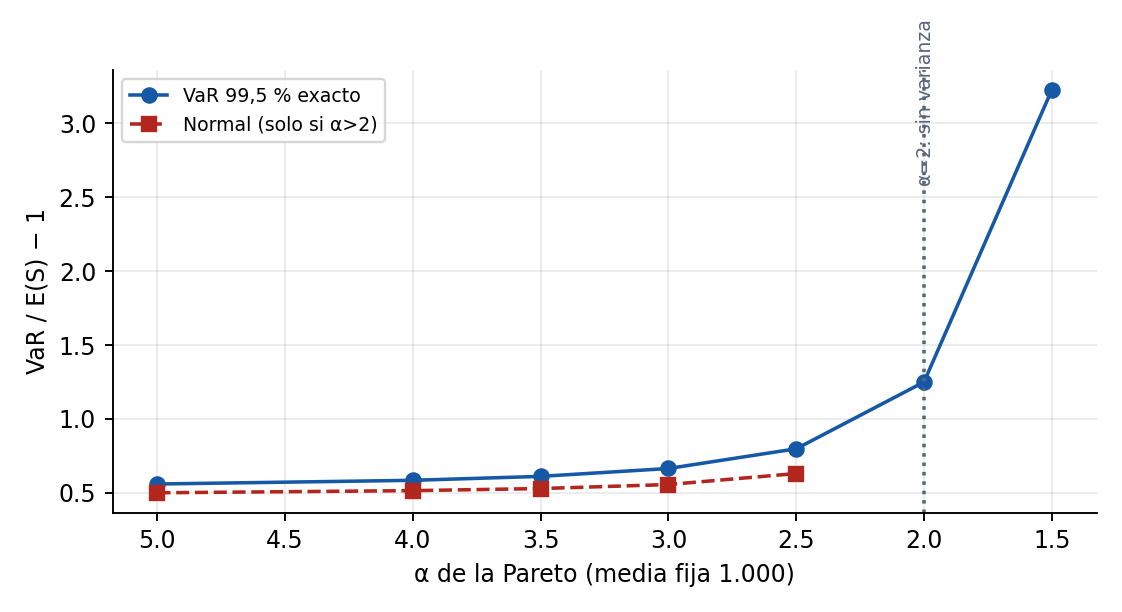
\includegraphics[width=.72\linewidth]{t3_f_debate3.png}
\caption{El capital exacto se dispara al engordar la cola; la Normal sigue una l\'inea casi plana y desaparece para $\alpha\le2$.}
\end{figure}
La Normal ``ve'' un capital casi constante porque depende de $\Var(S)$, que apenas cambia entre $\alpha=5$ y $\alpha=2{,}5$, y es incapaz de ver la cola. Para $\alpha\le2$ no puede dar ning\'un n\'umero, pero un analista que estime la varianza muestral s\'i obtiene uno: la varianza muestral de una Pareto con $\alpha=1{,}8$ pasa de $3{,}7\cdot10^6$ ($n=100$) a $7{,}2\cdot10^7$ ($n=100.000$), es decir, \emph{no converge}; la Normal resultante ser\'ia arbitraria y optimista.

\paragraph{3. Riesgos concretos.}
\begin{itemize}[leftmargin=*,itemsep=1pt]
\item \textbf{Infracapitalizaci\'on silenciosa}: el SCR calculado con la Normal subestima por mucho la p\'erdida del percentil 99,5\,\%, y el error crece justo cuando m\'as importa (colas pesadas: RC, incendio industrial, grandes siniestros).
\item \textbf{Inestabilidad del estimador}: la desviaci\'on t\'ipica muestral depende de la mayor observaci\'on; el capital cambiar\'ia mucho de un a\~no a otro.
\item \textbf{Dominio de un solo siniestro}: para colas pesadas $P(S>x)\approx\E[N]\,P(X>x)$ y $VaR_p\approx F_X^{-1}(1-(1-p)/\E[N])+\E[S]$. Con $\alpha=1{,}5$ da $632.245$ (exacto $633.750$): el capital es el cuantil de \emph{un} siniestro, no una propiedad de la suma.
\item \textbf{Diversificaci\'on ilusoria}: con varianza infinita aumentar la cartera no reduce el riesgo relativo a la velocidad $1/\sqrt n$; la reducci\'on es mucho m\'as lenta y puede no existir en capital.
\item \textbf{Medida de riesgo}: el TVaR es varias veces el VaR ($1{,}42$ M\euro\ frente a $0{,}63$ M\euro\ con $\alpha=1{,}5$); el SST (Expected Shortfall) exigir\'ia mucho m\'as que Solvencia~II.
\item \textbf{Riesgo de modelo y de estimaci\'on}: pasar de $\alpha=2$ a $1{,}5$ casi duplica el capital; y $\alpha$ se estima con error $\approx\alpha/\sqrt n$.
\end{itemize}

\paragraph{4. Qu\'e hacer.} Panjer/FFT o simulaci\'on con la severidad completa, EVT para la cola (Tema~5), reaseguro de exceso de p\'erdida que acote la severidad retenida, l\'imites de p\'oliza y m\'argenes de prudencia por incertidumbre en $\alpha$.

\bigskip\hrule\bigskip

\subsection{Debate 4 -- ?`Cu\'ando es preferible el modelo individual en una cartera grande de Generales?}

\paragraph{Tesis.} El colectivo es el est\'andar en Generales por su agilidad y porque, con Poisson, es matem\'aticamente robusto a la heterogeneidad. Hay casos en los que el individual aporta algo que el colectivo no puede:

\paragraph{1. Hipótesis de i.i.d. de la severidad que no se sostienen.}
\begin{itemize}[leftmargin=*,itemsep=1pt]
\item \textbf{Grandes riesgos identificables} (industria, transporte mar\'itimo, edificios singulares): cada uno tiene su propio capital asegurado, su l\'imite y su probabilidad de siniestro; no se parecen entre s\'i ni a la cartera atritional. Un colectivo les asigna una severidad com\'un y desdibuja que hay, por ejemplo, 20 riesgos de $5$ M\euro\ con $q=0{,}2\%$: el individual los trata uno a uno con su l\'imite.
\item \textbf{Severidad acotada por p\'oliza} (capital fijo en vida y accidentes; l\'imites de p\'oliza): el colectivo mezcla todas las severidades y puede dar probabilidad positiva a cuant\'ias superiores al l\'imite de la p\'oliza que las origina.
\item \textbf{Un solo siniestro posible por p\'oliza} (fallecimiento, invalidez, cancelaci\'on): el colectivo (Poisson) permite varios, y esto pesa cuando $q$ no es peque\~na (diferencia $\sum q_i^2\mu_i^2$ en varianza; $+5{,}3\%$ en Accidentes con $q$ de $5$--$8\%$).
\end{itemize}

\paragraph{2. Decisiones por p\'oliza.} Suscripci\'on, recargos de seguridad, reaseguro \emph{por riesgo} y asignaci\'on de capital necesitan la contribuci\'on de cada p\'oliza a $\E[S]$ y $\Var(S)$: eso es el modelo individual ($q_i b_i$ y $q_i(1-q_i)b_i^2$). Un colectivo no distingue entre p\'olizas.

\paragraph{3. Datos y trazabilidad.} Si se dispone de $q_i$ calibradas por un GLM p\'oliza a p\'oliza, el individual aprovecha toda esa informaci\'on; el colectivo la promedia. Modelos internos con exigencias de trazabilidad (EIOPA) pueden preferir un enfoque por p\'oliza en las l\'ineas m\'as singulares.

\paragraph{4. Un matiz que conviene reconocer.} La heterogeneidad \emph{en s\'i misma} no justifica el individual si la frecuencia es Poisson: la suma de Poisson compuestos independientes es un Poisson compuesto con $\lambda=\sum\lambda_j$ y severidad mezcla ponderada, de modo que el colectivo reproduce exactamente $\E[S]$ y $\Var(S)$ de la cartera heterog\'enea (as\'i lo comprueba la hoja de los cuatro segmentos: $\Var=1{,}715\cdot10^9$ en ambos c\'alculos). El colectivo pierde informaci\'on cuando hay sobredispersi\'on (heterogeneidad no observada) o cuando la composici\'on cambia y hay que re-estimar la mezcla.

\paragraph{5. Soluci\'on en la pr\'actica: un modelo h\'ibrido.} Colectivo para la cartera atritional, individual (o modelo de grandes siniestros con frecuencia y severidad propias) para los riesgos singulares, y agregaci\'on por convoluci\'on o por simulaci\'on con dependencia entre componentes.

\paragraph{Conclusi\'on.} En una cartera grande de Generales el individual compensa cuando hay pocos riesgos grandes y distintos entre s\'i, severidad acotada por p\'oliza, un siniestro m\'aximo por p\'oliza o decisiones por riesgo; en el resto, el colectivo con Poisson (o BN) es exacto y mucho m\'as eficiente.

\subsubsection*{Referencias}
\begin{itemize}[leftmargin=*,itemsep=0pt]
\item Klugman, S. A., Panjer, H. H. y Willmot, G. E. \emph{Loss Models: From Data to Decisions}. Wiley.
\item Cameron, A. C. y Trivedi, P. K. (2013). \emph{Regression Analysis of Count Data} (2.\textordfeminine\ ed.). Cambridge University Press.
\item Kaas, R., Goovaerts, M., Dhaene, J. y Denuit, M. (2008). \emph{Modern Actuarial Risk Theory} (2.\textordfeminine\ ed.). Springer.
\item Dutang, C., Goulet, V. y Pigeon, M. (2008). actuar: An R package for actuarial science. \emph{Journal of Statistical Software}, 25(7).
\item Directiva 2009/138/CE (Solvencia~II) y Reglamento Delegado (UE) 2015/35.
\end{itemize}

\end{document}
